\documentclass[12pt, a4paper]{report}

\usepackage{fyp}

\usepackage{graphicx}

%% for interactive URLS
\usepackage{hyperref}

%% for footnote refs
\usepackage{footmisc}
\interfootnotelinepenalty=10000

%% for inline code 
\usepackage{listings}
\lstset{
    basicstyle = \ttfamily,
    breaklines = true,
}

%%%%%%%%%%%%%%%%%%%%%%%%%%%%%%%%%%%%%%%%%%%%%%
                %%COMMENTING%%
%%%%%%%%%%%%%%%%%%%%%%%%%%%%%%%%%%%%%%%%%%%%%%
%% for commenting
\usepackage{soul}
\usepackage[dvipsnames]{xcolor}
% We also use DeclareRobustCommand instead of
% NewCommand so that the command will work in captions
% and other contexts as well.
\DeclareRobustCommand{\andre}[1]{ {\begingroup\sethlcolor{BurntOrange}\hl{(andre:) #1}\endgroup} }
\DeclareRobustCommand{\neville}[1]{ {\begingroup\sethlcolor{BurntOrange}\hl{(neville:) #1}\endgroup} }

%%%%%%%%%%%%%%%%%%%%%%%%%%%%%%%%%%%%%%%%%%%%%%
            %%LATEX DRAWINGS%%
%%%%%%%%%%%%%%%%%%%%%%%%%%%%%%%%%%%%%%%%%%%%%%
\usepackage{tikz}
\usepackage{tkz-euclide}
\usetikzlibrary{shapes,arrows,positioning}
\usetkzobj{}
%\usetkzobj{all}
%%%%%%%%%%%%%%%%%%%%%%%%%%%%%%%%%%%%%%%%%%%%%%

%%these packages are not really necessary if you dont need the code and proofs environments
%%so if you like you can delete from here till the next comment
%%note that there are some examples below which obviously won't work once you remove this part
\usepackage{verbatim}
\usepackage{amsfonts}
\usepackage{amsmath}
\usepackage{amssymb}
\usepackage{amsthm}

%%this environment is useful if you have code snippets
\newenvironment{code}
{\footnotesize\verbatim}{\endverbatim\normalfont}

%%the following environments are useful to present proofs in your thesis
\theoremstyle{definition}
\newtheorem{definition}{Definition}[section]
\theoremstyle{definition}%plain}
\newtheorem{example}{Example}[section]
\theoremstyle{definition}%remark}
\newtheorem{proposition}{Proposition}[section]
\theoremstyle{definition}%remark}
\newtheorem{lemma}{Lemma}[section]
\theoremstyle{definition}%remark}
\newtheorem{corollary}{Corollary}[section]
\theoremstyle{definition}%remark}
\newtheorem{theorem}{Theorem}[section]
%%you can delete till here if you dont need the code and proofs environments



\setlength{\headheight}{15pt}
%\overfullrule=15pt


\begin{document}

%%make sure to enter this information
\title{Program Analysis: Towards the Analysis of CPython Bytecode}
\author{André Theuma}
\date{22/04/2022}
\supervisor{Dr. Neville Grech}
\department{Faculty of ICT}
\universitycrestpath{uom-logo}
\submitdate{27/05/2022} 

\frontmatter

\begin{acknowledgements}
your acknowledgements
\end{acknowledgements}
       
\begin{abstract}
    \andre {Reworked abstract}
    \par Program analysis methods offer static compile-time techniques to predict approximations to a set of values or dynamic behaviours which arise during a program's run-time.
    These methods generate useful observations and characteristics about the underlying program, in an automated way.
    \par PATH (Python Analysis Tooling Helper) is a static analysis tool created in this project, which generates a standardized Intermediary Representation for 
    given functions, allowing analysis metrics to be generated from the facts produced by the tool. The goal of this project was to create a framework that generates facts from a function, in addition to an IR that is amenable for further analysis.
    The framework created should simplify the engineering complexity of fact analysis for future use. PATH would disassemble CPython bytecode into a more 
    straightforward representation, making any further possible analyses a simpler task, as analysis can be conduced on the generated IR.
    \par The final findings of the project indicate that performing analysis on the IR generated by PATH is indeed a simpler task than generating facts manually and conducting block analysis without such a framework.
    These results are satisfactory and hold up to the aims of this project.

    \begin{figure}
        \centering
         %% flowchart
         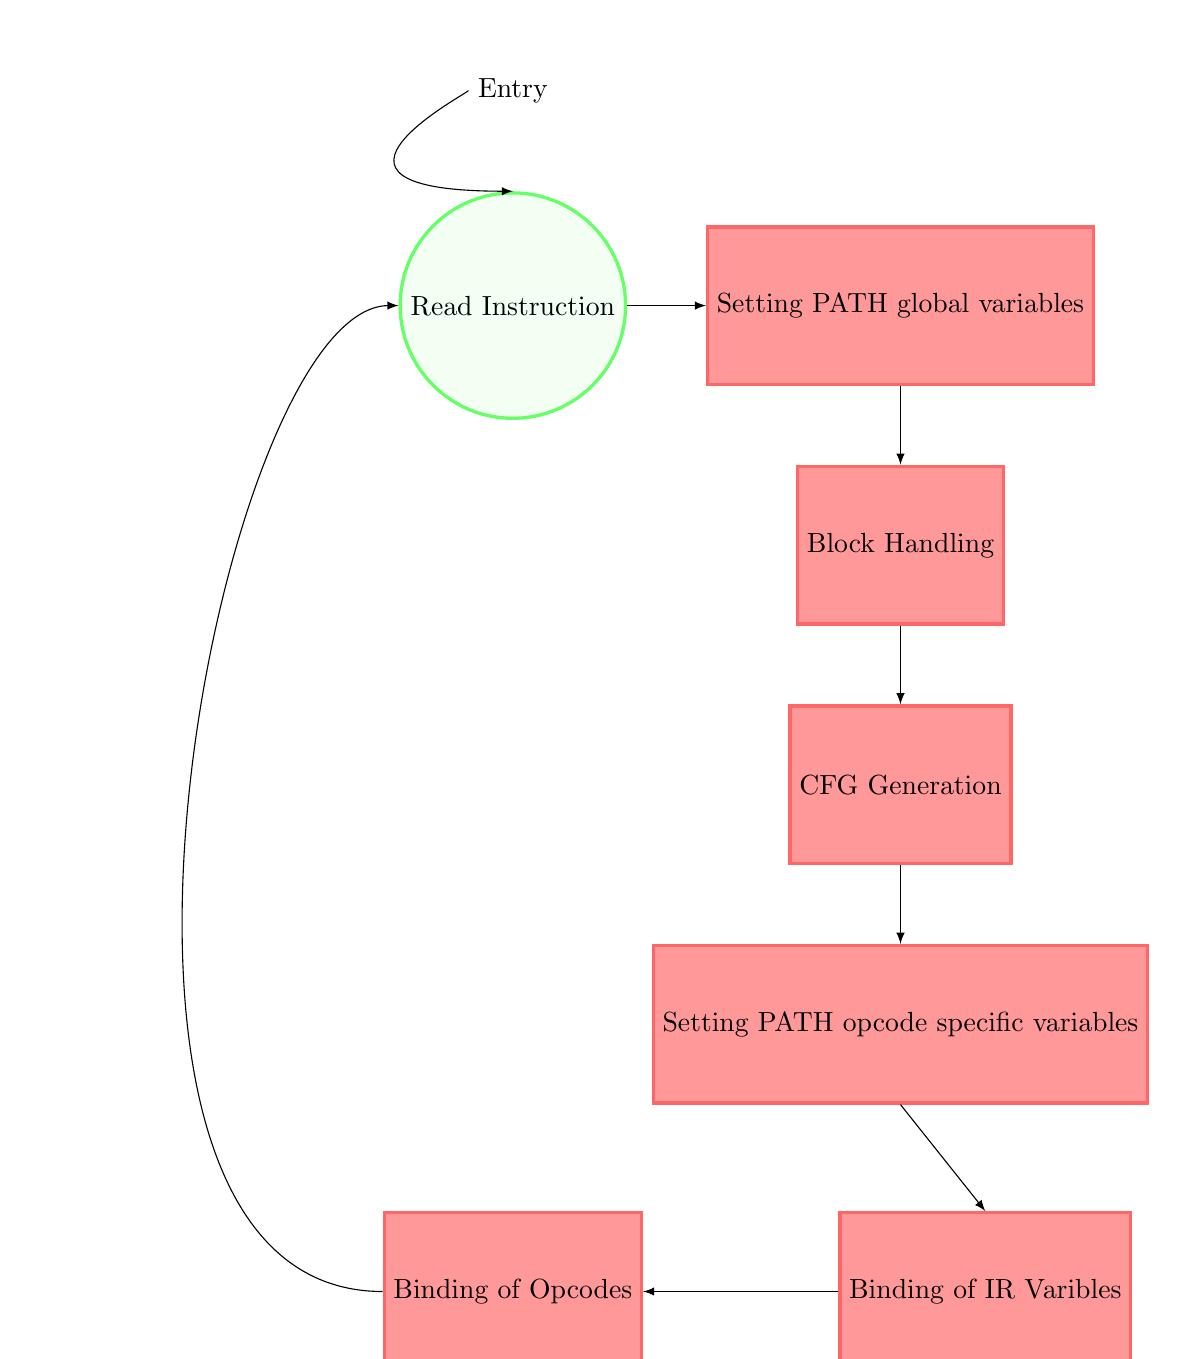
\begin{tikzpicture}
             %% setup
             [
                 roundnode/.style={circle, draw=green!60, fill=green!5, very thick, minimum size=20mm},
                 rectanglenode/.style={rectangle, draw=red!60, fill=red!40, very thick, minimum size=20mm},
                 transparentbox/.style={rectangle,draw=blue!60, fill=blue!0, ultra thick, minimum width = 75mm, minimum height = 40mm},
             ]
                 
                 %% Nodes
                 \node [roundnode] (instrRead) {Read Instruction};
                 \node [rectanglenode] (setvars) [right=of instrRead] {Setting PATH global variables};
                 \node [rectanglenode] (blockhandling) [below=of setvars] {Block Handling};
                 \node [rectanglenode] (cfg) [below=of blockhandling] {CFG Generation};
                 \node [rectanglenode] (opcodehandler) [below=of cfg] {Setting PATH opcode specific variables};
                 \node [rectanglenode] (opcodeBinding) [below=of opcodehandler] at(0,-10.5) {Binding of Opcodes};
                 \node [rectanglenode] (irbinding) [below=of opcodehandler] at(6,-10.5) {Binding of IR Varibles};

                 
                \node [] (entrytext) [above=of instrRead] {Entry};

                 %% Lines
                 \draw[-latex] (entrytext) .. controls +(left:.5cm) and +(left:3cm) .. (instrRead.north);
                 \draw[-latex] (instrRead.east) -- (setvars.west);
                 \draw[-latex] (setvars.south) -- (blockhandling.north);
                 \draw[-latex] (blockhandling.south) -- (cfg.north);
                 \draw[-latex] (cfg.south) -- (opcodehandler.north);
                 \draw[-latex] (opcodehandler.south) -- (irbinding.north);
                 \draw[-latex] (irbinding.west) -- (opcodeBinding.east);
                
                 \draw[-latex] (opcodeBinding.west) .. controls +(left:4.5cm) and +(left:2.3cm) .. (instrRead.west);

                 
                
        
        \end{tikzpicture}
         
        \caption{PATH High-Level Overview}
        \label{fig:python code execution}
     \end{figure}
 
   
\end{abstract}

\tableofcontents

\listoffigures

\listoftables



\mainmatter

\chapter{Introduction}

\andre{Reworked Introduction}

\par As an increasing number of people are becoming reliant on complex software systems, the lack of security and analysis
tooling frameworks is unacceptable in this day and age. Such frameworks provide vital insight for software systems;
allowing further development and refinement of the said system. Core vulnerabilities may be exposed and optimizations can be implemented.
Tools such as Pylint \cite{pylint2021}, and Bandit \cite{bandit2022} already exist in the industry.

\par PATH (Python Analysis Tooling Helper) provides general metrics for functions; known as facts, along with a
 standardized IR (Intermediary Representation) for external analysis. PATH also creates a Control Flow Graph for flow analysis.

    \section{Preliminary Overview}
        \subsection{Python \& CPython}
        \andre{Reworked}
        \par Python is a high-level, object-oriented scripting language \cite{lutz2001programming}, 
        suited for a wide range of development domains; from text processing \cite{bonta2019comprehensive} to 
        machine learning \cite{tensorflowTour} to game development \cite{sweigart2012making}. 
        The language's wide adoption (TIOBE's Language of the Year: 2007, 2010, 2018, 2020, 2021; \cite{tiobe2022index}) 
        may be attributed to the fact that it is based on the English language \cite{saabith2019python}, 
        making it easy to learn; aiding in the production of relatively complex programs. It is used extensively for rapid prototyping,
        as well developing fully-fledged real-world applications.

        \par The most common and comprehensive implementation of Python is known as CPython \cite{van2021python}; a bytecode interpreter for Python, written in C.

        \subsection{Program Analysis}
        \andre{Reworked}
        \par Complex programs imply complex behaviours. Such behaviours have to be analysed, as they might
        highlight certain vulnerabilities, and possibly indicate where optimizations can be carried out in the program.
        This area of interest is known as Program Analysis. Program Analysis provides answers for the following questions;
        \begin{itemize}
            \item Can the provided code be optimized?
            \item Is the provided code free of errors?
            \item How does data flow through the program \& in what order do instructions get executed (Control-Flow)?
        \end{itemize}
        \andre{Reworked}
        \par Naturally, as an increasing amount of modern day systems and frameworks are developed in Python, the need for properly conducting program analysis on these systems is ever-growing.
        There are two main approaches regarding program analysis; Dynamic Program Analysis \& Static Program Analysis. Dynamic analysis is the testing and evaluation of 
        an application during runtime, whilst static analysis is the testing and evaluation of an application by examining the code, producing facts and deducing
        possible errors in the program from the facts produced; without code execution \cite{intel2013analysis}. Since all (significant) properties of the 
        behaviour of programs written in today's' programming languages are mathematically undecidable \cite{rice1953classes}, one must involve approximation
        for an accurate analysis of programs. This kind of analysis cannot be carried out by a Dynamic analysis as carrying out a runtime
        analysis only reveals errors, but does not show the absence of errors \cite{moller2012static}; being the main motivation behind Static analysis. With the 
        right kind of approximations, Static analysis provides guarantees regarding properties of all the possible execution paths
        a program can take, giving it a clear advantage over Dynamic analysis; thus will be the main topic of interest in this paper. 
        
    \section{Aims \& Objectives}
    \andre{Reworked}
    \par The essential aim of this dissertation is the production of an analytical tool (PATH) which can be easily implemented in existing software systems.
    The tool is to be used on Python V3.10 \cite{van2021python} systems which are interpreted with the CPython \cite{van2021python} interpreter. It needs 
    to scale up to larger systems, and still provide accurate metrics. The analytical tool must also generate a standardized IR of the functions 
    present in the system being analysed. The standardized IR that is generated has to summarize the block analysis that is done by PATH. 
    \par The creation of this tool is vital as there is a lack of security and analysis tooling, for what is the worlds most used programming language 
    \cite{tiobe2022index};  giving developers an increased freedom of choice when having to choose an analysis framework for their projects.
    
    \section{Chapters Overview}
    This paper is composed of five chapters, which can be broken down in the following manner:
    \par Chapter 1 contains the introductory content, along with a brief overview of the technologies and ideas that are going to be delved into further
    along the paper. The introduction also gives a run-down of the main objectives that are to be met in this project.
    \par Chapter 2 gives an in-depth literature review of the content that is briefly touched upon in the introductory chapter [Chapter 1]. The literature review
    consists of (but is not limited to) the following works; Python, the uses of Python, Python's bytecode \& CPython's \textit{ceval.c} interpreter, and Static Analysis Tooling.
    \par Chapter 3 delves into the methodology and implementation of the disassembler (PATH). The design of choice is further discussed together with the reasons for ongoing into 
    such a design are highlighted.
    \par Chapter 4 evaluates the results produced by PATH and answers specific research questions, ensuring that the Analytical toolkit works as intended. A couple of case-studies are included
    testing the scalability and ease-of use of PATH.
    \par Chapter 5 presents the conclusions of the project and any suggestions for further work that can be done.

    \andre{New}
    \section{Contributions}
    \par A.T carried out the reverse engineering of the individual CPython bytecodes; observing their effect on the value stack. These operations are concisely noted
    in the \nameref{table:opcode_table}.
    \par A.T automated the production of facts from Python functions, expediting different analyses of functions.
    \par A.T standardized the generation of an IR; exposing to the user for better understanding of function behaviours. Alongside IR generation, control flow with functions
    is indicated by a Control-Flow graph. 


\chapter{Background \& Literature Review}
    \section{Python}
        \subsection{History}
        \par Python being a general-purpose \cite{srinath2017python}, high-level programming language \cite[pp.2--4]{van1995python}, makes the development of complex software systems a relatively non-trivial task
        in comparison to the production complexity that comes along with other comparable programming languages, such as C \cite{summerfield2007rapid}.
        \par The language was developed to be a successor of the ABC programming language \cite{geurts1990abc} and was initially released as Python V0.9.0 in 
        1991. Similarly to ABC, Python has an English-esque syntax but differs in its application domain; Python being a tool that is intended to be used in a more professional environment, whilst
        ABC is geared towards non-expert computer users \cite[pp.285--288]{van1991interactively}. 
        
        \subsection{Features \& Philosophy}
        \par The simplicity of Python enables it to be an extremely popular language to use in the industry of software development \cite{tiobe2022index}. It was designed with the intention
        to be highly readable, thus removing the 'boilerplate' style used in the more traditional languages, such as Pascal. Python uses indentation for block delimiters,
        (off-side rule \cite[pp.4--5]{van2021python}) which is unusual among other popular programming languages \cite[pp.2--3]{van2021python}; new blocks increase in indentation, whilst the end of 
        a current block is signified by the decrease of an indentation. It supports a dynamic type system, enabling the compiler to run faster and the CPython interpreter to dynamically load new code. 
        Dynamic type systems such as Python offer more flexibility; allowing for simpler language syntax, which in turn leads to a smaller source code size \cite{dynamic2013typing}. Although dynamically typed,
        Python is also strongly-typed; disallowing operations which are not-well defined. Objects are typed albeit variable names are untyped.
        \andre{Reworked}
        \par One of Python's most attractive features is that it offers the freedom to allow the developer to use multiple programming paradigms \cite{van2007python}; appealing to a wider audience. Python
        also includes a cycle-detecting garbage collector \cite{van2007python}, freeing up objects as soon as they become unreachable \cite[pp.9--10]{van1994python}. Objects are not explicitly freed up
        as the collector requires a significant processing overhead \cite[pp.27-30]{zorn1990barrier}, and re-allocating memory to objects every time an object is required is resource consuming. Python has 
        module support in its design philosophy formulating a highly extensible language. Modules can be written in C/C++ \cite{srinath2017python} and imported as libraries in any Python project;
        highlighting the extensibility of the language. There are plenty \footnote{Over 329,000 packages as of September 2021 \cite{van2007python}} of readily available 
        third-party libraries suited for many tasks, ranging from Web Development \cite{forcier2008python} to complex Machine Learning frameworks \cite{pedregosa2011scikit}, further increasing 
        ease-of use, and supporting the quick and simple development philosophy of Python.

        \subsection{Implementations}
        \par There are several environments which support the Python language; known as implementations. The default, most feature comprehensive Python implementation is 
        CPython\footnote{The terms CPython and Python are typically used interchangeably. This will be the case in this paper, unless specified otherwise.} \cite{vanrossum1995python} ,written and maintained by Guido van Rossum. Other popular re-implementations include PyPy \cite{bolz2009tracing}, 
        Jython \cite{juneau2010definitive} and IronPython \cite{mueller2010professional}. This paper will focus on the CPython implementation of the Python language and
        will not cover any of the other alternate implementations.

    \section{CPython}
        \subsection{Overview}
        \andre{Reworked}
        \par CPython is the predominant implementation of the Python language, and is written in C. It has a thin compilation layer from source code to CPython bytecode (See \ref{fig:compiler_innards}); simplifying the design of the interpreter.
        Unlike the typical structured program representations, bytecode is easier to parse, and has a standardized notation.
        \par CPython works transparently, via the PVM(Python Virtual Machine \ref{fig:vm_innards}); an interpreter loop is run \footnote{\label{footnote:ceval}\textit{ceval.c}} and there is no direct translation between the Python code to C \cite[pp.1--2]{aycock1998converting}. 
        The PVM is known as a stack machine, whereby PVM instructions retrieve their arguments from the stack, just to be placed back onto the stack after the instruction is executed. It can be said that the Python compiler generates PVM code\footnote{PVM code is also known as a \textit{.pyc} file.} for the python VM to execute.
        The CPython interpreter resembles a classic interpreter with a straightforward algorithm \cite[pp.2--4]{aycock1998converting}: 
        \begin{itemize}
            \item[1.] Firstly, the opcode of a VM instruction is fetched, along with any necessary arguments.
            \item[2.] Secondly, the instruction is then executed.
            \item[3.] Finally, steps 1-2 are repeated till no more opcodes can be fetched. This is done by raising an exception when an invalid (empty) opcode is found.  
        \end{itemize}

        \begin{figure}
        \centering
            %% flowchart
            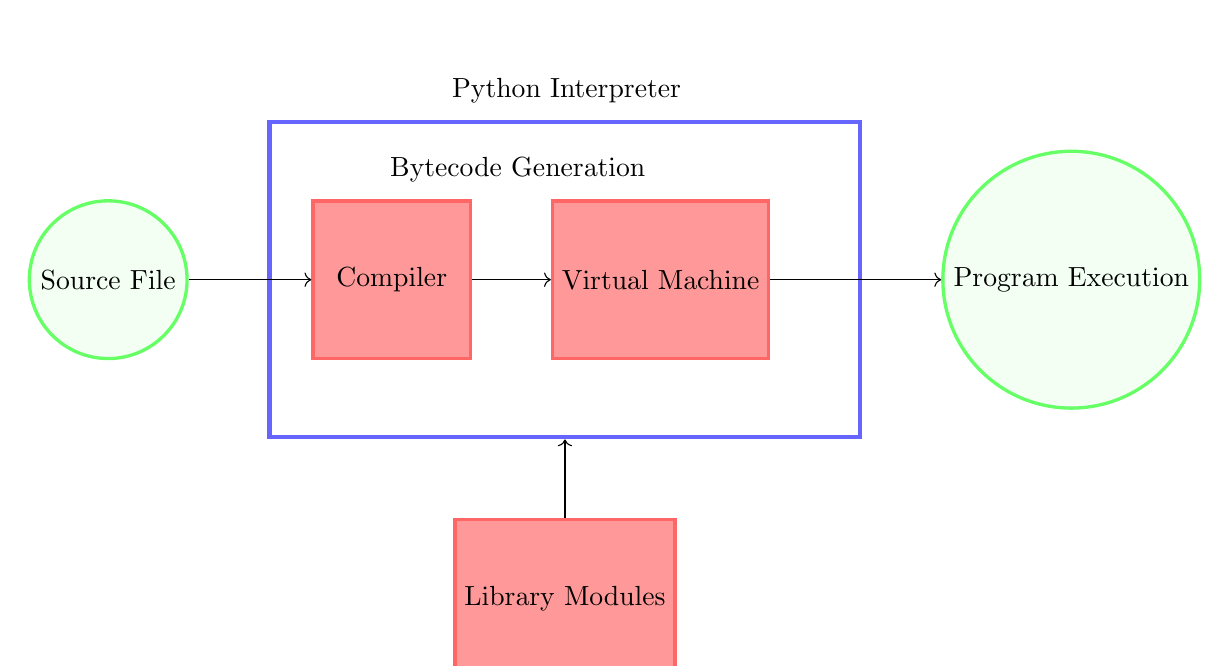
\begin{tikzpicture}
                %% setupP
                [
                    roundnode/.style={circle, draw=green!60, fill=green!5, very thick, minimum size=20mm},
                    rectanglenode/.style={rectangle, draw=red!60, fill=red!40, very thick, minimum size=20mm},
                    transparentbox/.style={rectangle,draw=blue!60, fill=blue!0, ultra thick, minimum width = 75mm, minimum height = 40mm},
                ]
                    
                    %% Nodes
                    \node [transparentbox] (box) at (1,0) {};
                    \node [rectanglenode] (compilernode) at (-1.2,0){Compiler};
                    \node [rectanglenode] (vmnode) [right=of compilernode] {Virtual Machine};
                    \node [roundnode] (sourcefile) [left=of box] {Source File};
                    \node [roundnode] (programnode) [right=of box] {Program Execution};
                    \node [rectanglenode] (librarynode) [below=of box] {Library Modules};
                    \node [] (text) at (1.02,2.4) {Python Interpreter};
                    \node [] (textBytecode) at (0.4,1.4){Bytecode Generation};
                    %% Lines
                    \draw[->] (librarynode.north) -- (box.south) ;
                    \draw[->] (sourcefile.east) -- (compilernode.west);
                    \draw[->] (compilernode.east) -- (vmnode.west);
                    \draw[->] (vmnode.east) -- (programnode.west);
                \end{tikzpicture}
            
                \caption{Python Code Execution}
                \label{fig:python code execution}
        \end{figure}

        \begin{figure}
            \centering    
            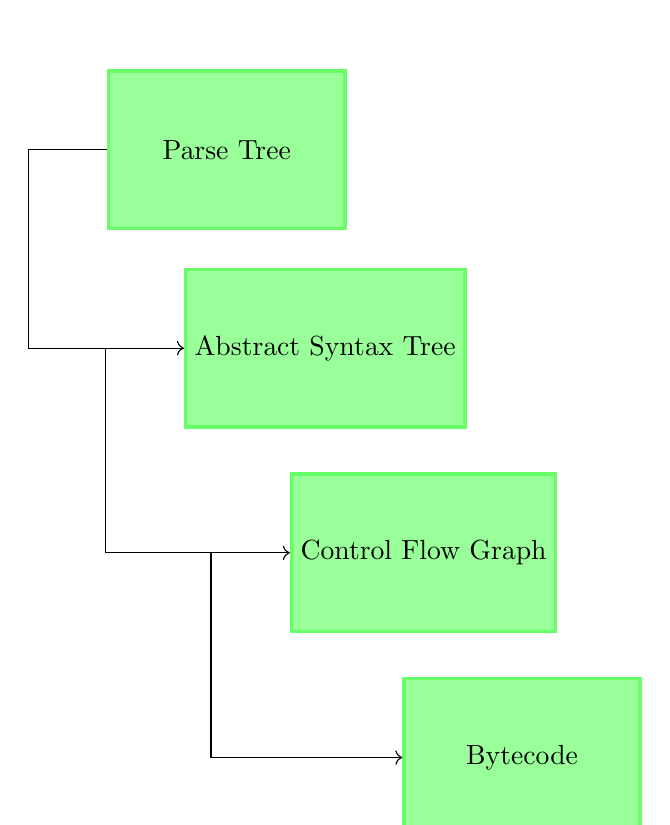
\begin{tikzpicture}
                [
                    roundnode/.style={circle, draw=green!60, fill=green!5, very thick, minimum size=20mm},
                    rectanglenode/.style={rectangle, draw=green!60, fill=green!40, very thick, minimum width=30mm, minimum height = 20mm},
                    transparentbox/.style={rectangle,draw=blue!60, fill=blue!0, ultra thick, minimum width = 75mm, minimum height = 40mm},
                ]
                
                \node [rectanglenode] (parsetree) {Parse Tree};
                \node [rectanglenode] (ast) [below=of parsetree] at(1.25,-0.5) {Abstract Syntax Tree};
                \node [rectanglenode] (cfg) [below=of ast] at(2.5,-3.1) {Control Flow Graph};
                \node [rectanglenode] (bytecode) [below=of cfg] at(3.75,-5.7) {Bytecode};

                \draw[->] (parsetree.west) -- ++(-1,0)|- (ast.west) ; 
                \draw[->] (ast.west) -- ++(-1,0)|- (cfg.west) ; 
                \draw[->] (cfg.west) -- ++(-1,0)|- (bytecode.west) ; 

            \end{tikzpicture}
            
            \caption{Compiler Innards}
            \label{fig:compiler_innards}
        \end{figure}

        \begin{figure}
            \centering
            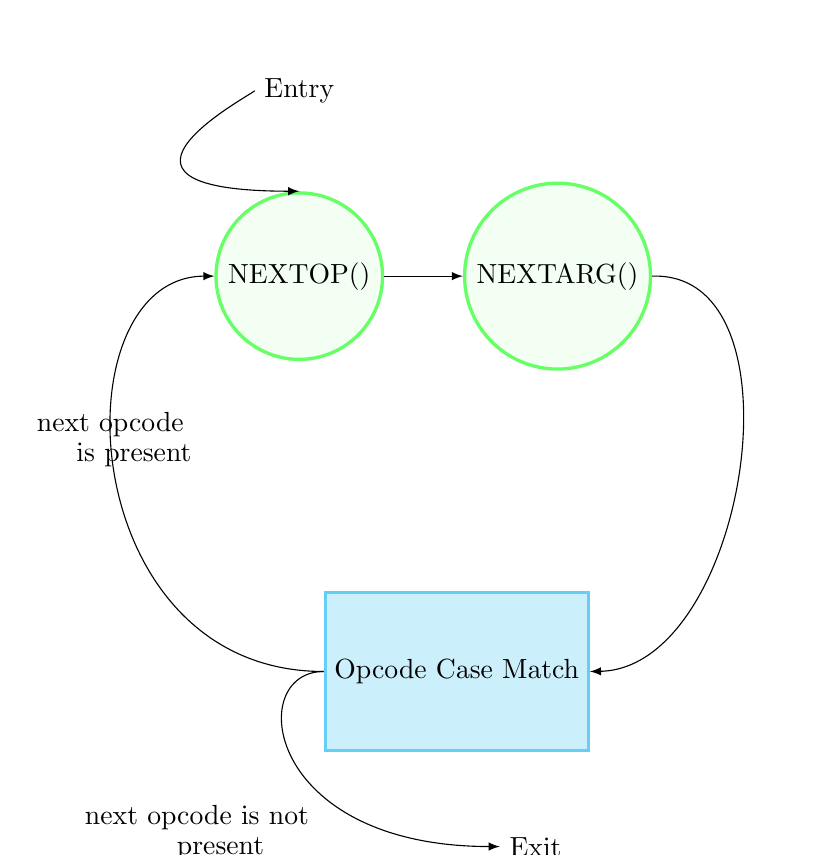
\begin{tikzpicture}
                [
                    roundnode/.style={circle, draw=green!60, fill=green!5, very thick, minimum size=20mm},
                    rectanglenode/.style={rectangle, draw=cyan!60, fill=cyan!20, very thick, minimum width=30mm, minimum height = 20mm},
                    transparentbox/.style={rectangle,draw=blue!60, fill=blue!0, ultra thick, minimum width = 75mm, minimum height = 40mm},
                ]

                \node [roundnode] (opcode) {NEXTOP()};
                \node [roundnode] (checkargs) [right=of opcode] {NEXTARG()};
                \node [rectanglenode] (switch) [below=of opcode] at(2,-3) {Opcode Case Match};
                \node [] (entrytext) [above=of opcode] {Entry};
                \node [] (exittext) [below=of switch] at(3,-6) {Exit};
                \node [] (label1) [below=of switch] at(-1.3,-5.6) {next opcode is not};
                \node [] (label1) [below=of switch] at(-1,-6) {present};
                \node [] (label2) [below=of switch] at(-2.4,-.6) {next opcode};
                \node [] (label2) [below=of switch] at(-2.1,-1) {is present};
                
                \draw[-latex] (entrytext) .. controls +(left:.5cm) and +(left:3cm) .. (opcode.north);
                \draw[-latex] (switch.west) .. controls +(left:1cm) and +(left:3cm) .. (exittext.west);
                \draw[-latex] (switch.west) .. controls +(left:3.2cm) and +(left:2cm) .. (opcode.west);
                \draw[-latex] (checkargs.east) to[in=1, out=2] (switch.east);
                
                \draw[-latex] (opcode.east) -- (checkargs.west);
                


            \end{tikzpicture}

            \caption{VM Innards}
            \label{fig:vm_innards}
        \end{figure}

        \pagebreak
        This simple algorithm is known as the CPython Evaluation Loop \footref{footnote:ceval}. The evaluation loop \footref{footnote:ceval} is formulated in the following 
        manner\footnote{Actual code differs from what is presented. The source code has been edited as to be more readable and concise.}:
        
        \begin{figure}
            \centering
            \begin{code}
                for(**indefinite condition**){
                    oparg=null;
                    opcode = NEXTOP();
                    if(ARGUMENT_PRESENT(opcode)){
                        oparg = NEXTARG();
                    }
                    switch(opcode){
                        case **opcode_name**: 
                            manipulate stack & set variables accordingly
                        ...
                        ...
                        ...
                        default: 
                            raise error
                    }
                }
                            
            \end{code}
            \caption{Evaluation Loop}
            \label{lst:ceval_loop}

            \end{figure}
            Evaluation is computed frame by frame (See {\bfseries\nameref{subsec:frames}}), with what is essentially a (very long) switch statement; reading every opcode and delegating accordingly.
            
        \subsection{Stacks}
        \label{subsec:stacks}
        \par A stack data structure is a dynamic structure that operates with a LIFO policy \cite{intro2009algorithms}. Since CPython does not directly interact with
        the hardware for compilation, it makes both the call stack and stack frames rely on the PVM. In CPython there is one main stack that the PVM requires for proper functionality; the call stack. 
        The other two stacks (\nameref{subsubsec:value_stack} and \nameref{subsubsec:call_stack}) are essential for the proper computation of any variables that there are in the
        frame (See {{\bfseries\nameref{subsec:frames}}). Most instructions manipulate the value stack and the call stack \cite{general2018stacks}.
            \andre{Reworked}
            \subsubsection*{Call Stack}
            \label{subsubsec:call_stack}
            \par The call stack contains call-frames\footref{footnote:call-frame_def} (See {\bfseries\nameref{subsec:frames}}). This is the main structure of the running program.
            A function call results into a pushed frame onto the call stack whilst 
            a return call results into a pop of the function frame off of the stack \cite{call2010stack}. A visual representation of a call stack is shown in Figure \ref{fig:call_stack_example}. 
            In this figure a sample script can be seen run, step by step, showing the frames being pushed onto the call stack and popped from the call stack.
            The first frame pushed onto the frame stack is inevitably called the \lstinline|__main__| call frame.
            
            \begin{figure}
                \centering
                {\bfseries Python Test Script}
                

                \begin{code}
                def foo():
                    print("Hello")
                
                def intermediary():
                    foo()
                    
                def start():
                    intermediary()
                
                start()
                \end{code}

                \label{lst:call_stack_example}
                
                %%TODO: FIX SIZE
                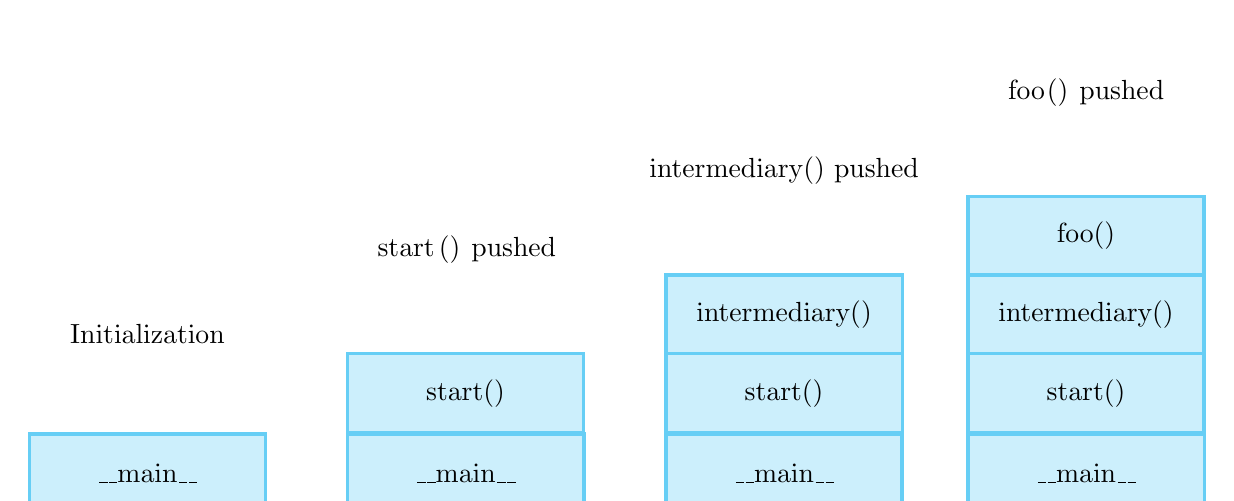
\begin{tikzpicture}
                [
                    roundnode/.style={circle, draw=green!60, fill=green!5, very thick, minimum size=20mm},
                    rectanglenode/.style={rectangle, draw=cyan!60, fill=cyan!20, very thick, minimum width=30mm, minimum height = 10mm},
                    transparentbox/.style={rectangle,draw=blue!60, fill=blue!0, ultra thick, minimum width = 75mm, minimum height = 40mm},
                ]
                
                \node[rectanglenode] (main) at (0,0) {\_\_main\_\_};
                \node [] (text_init) [above=of main] {Initialization};
                
                \node[rectanglenode] (main_1) [right=of main] {\_\_main\_\_};
                \node[rectanglenode] (start) [above=of main_1] at (4.04,-0.5) {start()};
                \node [] (text_start) [above=of start] {\lstinline|start()| pushed};

                \node[rectanglenode] (main_2) [right=of main_1] {\_\_main\_\_};
                \node[rectanglenode] (start_2) [above=of main_2] at (8.085,-0.5) {start()};
                \node[rectanglenode] (intermediary) [above=of start_2] at(8.085,0.5) {intermediary()};
                \node [] (text_int) [above=of intermediary] {\lstinline|intermediary()| pushed};
            
                \node[rectanglenode] (main_3) [right=of main_2] at (9.40,0){\_\_main\_\_};
                \node[rectanglenode] (start_3) [above=of main_3] at (11.92,-0.5) {start()};
                \node[rectanglenode] (intermediary_3) [above=of start_3] at(11.92,0.5) {intermediary()};
                \node[rectanglenode] (foo) [above=of intermediary_3] at(11.92,1.5) {foo()};
                \node [] (text_foo) [above=of foo] {\lstinline|foo()| pushed};

                \end{tikzpicture}
                
                \vspace{40mm}

                %%TODO: FIX SIZE
                \begin{tikzpicture}
                    [
                        roundnode/.style={circle, draw=green!60, fill=green!5, very thick, minimum size=20mm},
                        rectanglenode/.style={rectangle, draw=cyan!60, fill=cyan!20, very thick, minimum width=30mm, minimum height = 10mm},
                        transparentbox/.style={rectangle,draw=blue!60, fill=blue!0, ultra thick, minimum width = 75mm, minimum height = 40mm},
                    ]
                    
                    \node[rectanglenode] (main) at (8.21,0) {\_\_main\_\_};
                    \node [] (text_init) [above=of main] {\lstinline|start()| popped};
                    
                    \node[rectanglenode] (main_1) [right=of main_2] at(1.86,0) {\_\_main\_\_};
                    \node[rectanglenode] (start) [above=of main_1] at (4.38,-0.5) {start()};
                    \node [] (text_start) [above=of start] {\lstinline|intermediary()| popped};
        
                    \node[rectanglenode] (main_2) [right=of main_3] at (-2.3,0){\_\_main\_\_};
                    \node[rectanglenode] (start_2) [above=of main_2] at (0.215,-0.5) {start()};
                    \node[rectanglenode] (intermediary) [above=of start_2] at(0.215,0.5) {intermediary()};
                    \node [] (text_int) [above=of intermediary] {\lstinline|foo()| popped};
                
                    \node[rectanglenode] (main_3) at (-3.6,0){\_\_main\_\_};
                    \node[rectanglenode] (start_3) [above=of main_3] at (-3.6,-0.5) {start()};
                    \node[rectanglenode] (intermediary_3) [above=of start_3] at(-3.6,0.5) {intermediary()};
                    \node[rectanglenode] (foo) [above=of intermediary_3] at(-3.6,1.5) {foo()};
                    \node [] (text_foo) [above=of foo] at (-3.6,2.5){\lstinline|foo()| computed};
        
                \end{tikzpicture}

                \caption{Call Stack}
                \label{fig:call_stack_example}

            \end{figure}

            \subsubsection*{Value Stack}
            \label{subsubsec:value_stack}
            \andre{Reworked}
            \par This stack is also known as the evaluation stack. It is where the manipulation of object happens when object-manipulating opcodes are evaluated.
            A value stack is found in a call-frame implying bijectivity. Any manipulations that are performed on this stack (unless they are namespace related) are independent of other stacks and
            do not have the permissions to push values on other value stacks.
            
            \subsubsection*{Block Stack}
            \label{subsubsec:block_stack}

            \par The block stack keeps track of different types of control structures, such as; loops, try/except blocks and with blocks. These structures push entries onto the block stack, which are popped whenever the
            said structure is exited. The block stack allows the interpreter to keep track of active blocks at any moment

            \begin{figure}
                \centering

                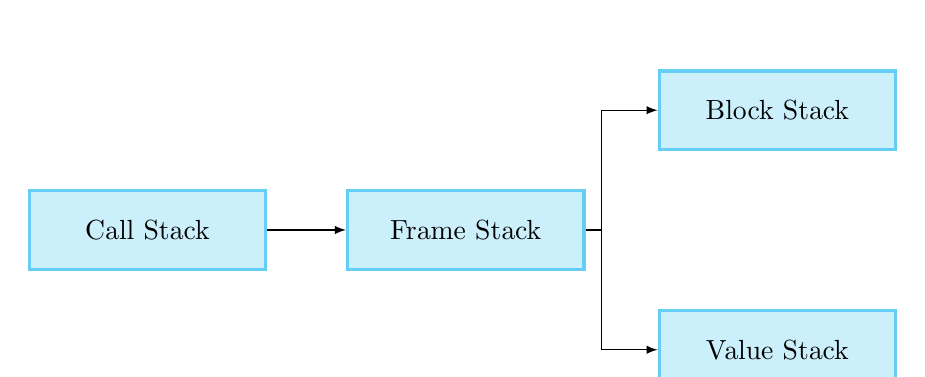
\begin{tikzpicture}
                    [
                        roundnode/.style={circle, draw=green!60, fill=green!5, very thick, minimum size=20mm},
                        rectanglenode/.style={rectangle, draw=cyan!60, fill=cyan!20, very thick, minimum width=30mm, minimum height = 10mm},
                        transparentbox/.style={rectangle,draw=blue!60, fill=blue!0, ultra thick, minimum width = 75mm, minimum height = 40mm},
                    ]

                    \node[rectanglenode] (callstack) at (0,0) {Call Stack};

                    \node[rectanglenode] (framestack) [right=of callstack] {Frame Stack};
                    \node[rectanglenode] (blockstack) [above=of framestack] at (8,0) {Block Stack};
                    \node[rectanglenode] (valuestack) [below=of framestack] at (8,0){Value Stack};
                    

                    \draw[-latex] (callstack) -- (framestack);
                    \draw[-latex] (framestack.east) -- ++(0.2,0)|-  (blockstack.west);
                    \draw[-latex] (framestack.east) -- ++(0.2,0)|-  (valuestack.west);

                \end{tikzpicture}

                \caption{Overview of CPython stacks}
                \label{fig:stacks_overview}
            \end{figure}

        \subsection{Frames}
        \label{subsec:frames}
        \andre{Maybe change???}
        \par A frame\footnote{\label{footnote:call-frame_def}Also called a call-frame.}, is an object which represents a current function call (subprogram call); more formally referred to as a code object. It is an internal type containing administrative information useful for debugging and is used internally
        by the interpreter \cite[pp.18--19]{van1994python}. Frame objects are tightly coupled with the three main stacks (See {\bfseries\nameref{subsec:stacks}}) and every frame is linked with another frame. Every frame object has two frame-specific stacks;
        value stack (See {\bfseries\nameref{subsubsec:value_stack}}) and the block stack (See {\bfseries\nameref{subsubsec:block_stack}}). Frames are born from function calls, and die when that function is returned.
        
            \subsubsection*{Frame Attributes}
            \par Along with the properties mentioned above, a frame object would have the following attributes \footnote{Retrieved from declaration found in \textit{./Include/frameobject.h}}:
            \begin{itemize}
                \item \lstinline|f_back|: this is\footnote{\label{footnote:frame_obj_attribs}In this context; "...this is..." or "...this holds..." does not mean the actual value is being stored in the variable, but a pointer to the address of the value is being stored.} the previous stack frame object (return address).
                \item \lstinline|f_code|: this is\footref{footnote:frame_obj_attribs} the current code object (See {\bfseries\nameref{subsec:code_obj}}) being executed, in the current frame.
                \item \lstinline|f_builtin|: this is\footref{footnote:frame_obj_attribs} the builtin symbol table.
                \item \lstinline|f_globals|: this is\footref{footnote:frame_obj_attribs} the dictionary used to look up global variables.
                \item \lstinline|f_locals|: this is\footref{footnote:frame_obj_attribs} the symbol table used to look up local variables.
                \item \lstinline|f_valuestack|: this is a pointer, which points to the address after the last local variable.
                \item \lstinline|f_valuestack|: this holds\footref{footnote:frame_obj_attribs} the value of the top of the value stack.
                \item \lstinline|f_lineno|: this gives the line number of the frame.
                \item \lstinline|f_lasti|: this gives the bytecode instruction offset of the last instruction called.
                \item \lstinline|f_blockstack|: contains the block state, and block relations.
                \item \lstinline|f_localsplus|: is a dynamic structure that holds any values in the value stack, for evaluation purposes.
            \end{itemize}

            \subsubsection*{Frame Stack}
            \andre{Reworked}
            \par The stack frame is a collection of all the current frames in a call-stack-like data structure (See {\bfseries\nameref{subsubsec:call_stack}}).
            A frame is pushed onto the stack frame for every function call (as typically, every function has its own unique frame) as shown in Figure \ref{fig:stack_frames}.
            \par The stack frame contains a frame pointer which is another register that is set to the current stack frame. Frame pointers resolve the issue that is created 
            when operations (pushes or pops) are computed on the stack hence changing the stack pointer, invalidating any hard-coded offset addresses that are computed statically, prior to run-time \cite{stack2011csuwm}.
            With frame pointers references to the local variables are made as offsets from the frame pointer not the stack pointer.
            \begin{figure}
                
                \centering
                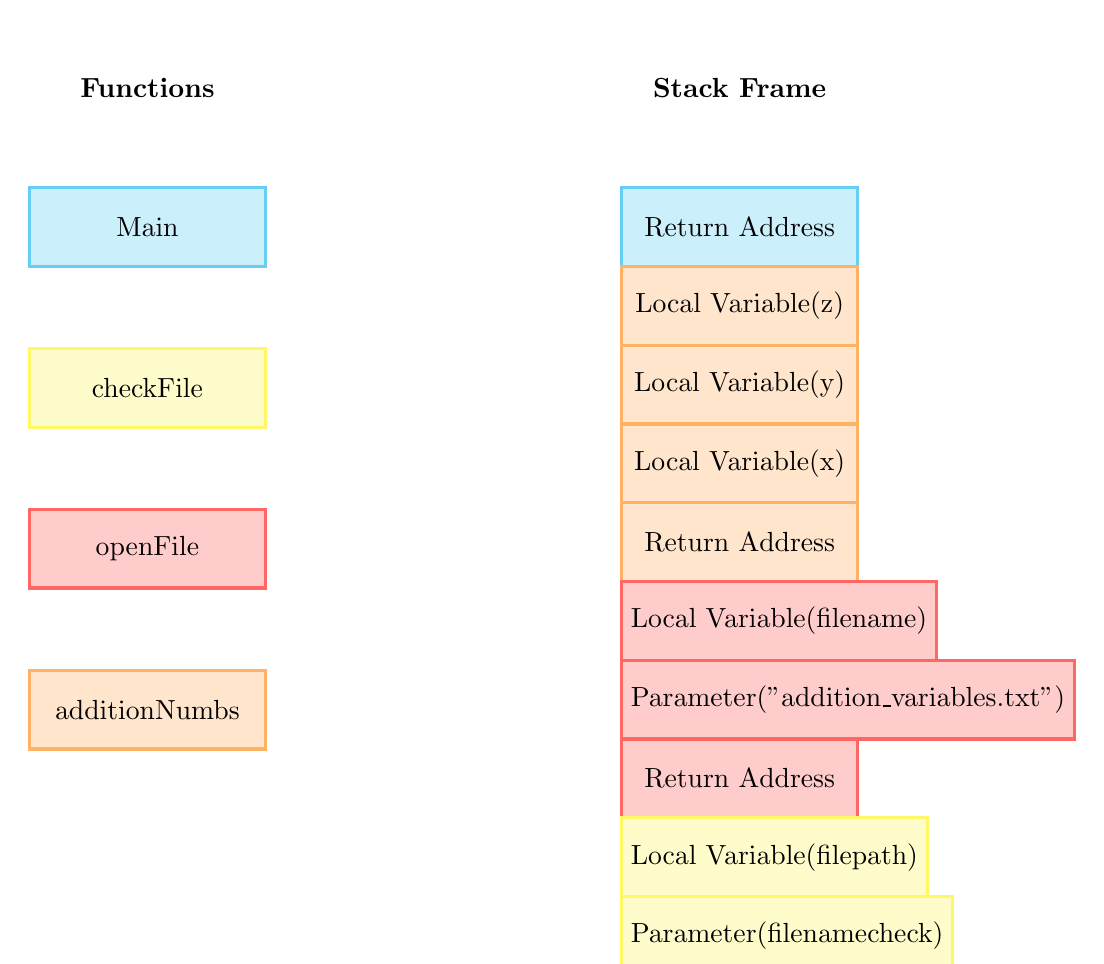
\begin{tikzpicture}
                    [
                        roundnode/.style={circle, draw=green!60, fill=green!5, very thick, minimum size=20mm},
                        rectanglenode_main/.style={rectangle, draw=cyan!60, fill=cyan!20, very thick, minimum width=30mm, minimum height = 10mm},
                        rectanglenode_checkFile/.style={rectangle, draw=yellow!60, fill=yellow!20, very thick, minimum width=30mm, minimum height = 10mm},
                        rectanglenode_openFile/.style={rectangle, draw=red!60, fill=red!20, very thick, minimum width=30mm, minimum height = 10mm},
                        rectanglenode_addition/.style={rectangle, draw=orange!60, fill=orange!20, very thick, minimum width=30mm, minimum height = 10mm},
                        transparentbox/.style={rectangle,draw=blue!60, fill=blue!0, ultra thick, minimum width = 75mm, minimum height = 40mm},
                    ]
                    
                    
                    \node[rectanglenode_main] (mainfunc) at (0,0) {Main};
                    \node[rectanglenode_checkFile] (func1) [below=of mainfunc] {checkFile};
                    \node[rectanglenode_openFile] (func2) [below=of func1] {openFile};
                    \node[rectanglenode_addition] (func3) [below=of func2] {additionNumbs};
                    
                    \node[rectanglenode_main] (mainfunc_frame1) [right= of mainfunc] at (5,0) {Return Address};
                    \node[rectanglenode_addition] (addition_frame1) [right= of mainfunc] at (5,-1) {Local Variable(z)};
                    \node[rectanglenode_addition] (addition_frame1) [right= of mainfunc] at (5,-2) {Local Variable(y)};
                    \node[rectanglenode_addition] (addition_frame1) [right= of mainfunc] at (5,-3) {Local Variable(x)};
                    \node[rectanglenode_addition] (addition_frame1) [right= of mainfunc] at (5,-4) {Return Address};
                    \node[rectanglenode_openFile] (openFile_frame1) [right= of func1] at(5,-5){Local Variable(filename)};
                    \node[rectanglenode_openFile] (openFile_frame2) [right= of func1] at(5,-6){Parameter("addition\_variables.txt")};
                    \node[rectanglenode_openFile] (openFile_frame3) [right= of func1] at(5,-7){Return Address};
                    \node[rectanglenode_checkFile] (checkFile_frame1) [right= of func1] at(5,-8){Local Variable(filepath)};
                    \node[rectanglenode_checkFile] (checkFile_frame2) [right= of func1] at(5,-9){Parameter(filenamecheck)};
                    
                    \node[] (textfunctions) [above=of mainfunc] {\bfseries{Functions}};
                    \node[] (textstack) [above=of mainfunc_frame1] {\bfseries{Stack Frame}};

                \end{tikzpicture}
                \caption{Stack frames example}
                \label{fig:stack_frames}
            
            \end{figure}

        \subsection{Code Objects}
        \label{subsec:code_obj}
        
        \par A code object is a low-level detail of the CPython implementation. When Python code is parsed, it is compiled into a code object to be run on the PVM. A code object contains a list of instructions which
        directly interact with the CPython VM; hence why it is called a low-level detail. Typically, code objects are of the type \lstinline|PyCodeObject|\footnote{\label{lst:pycodeobj}The type is the C structure of the object which is used to describe a code object.}
        and each section of the code object represents a chunk of executable code that has not been bound into a function \cite{pythonofficial2022docspycode}. The structure of the type of these code 
        objects \footref{lst:pycodeobj} change throughout different CPython versions, thus there is no set composition \cite{pythonofficial2022docspycode}. For reference, the source code in Figure \ref{lst:dis_example} produces
        the following code object: 
        \begin{code}
            <code object addition_numbers at 0x1047f10b0, file "filepath", line 3>
        \end{code}
        Which follows this convention:
        \small
        \begin{align}
            code object <functionName> at <address>, file <path>, line<firstLineNo.>
        \end{align}
        \normalsize

            \subsubsection*{Disassembler}
            \andre{Reworked}
            \par Code objects are expanded by using the \lstinline|dis| module in Python. This module contains several analyses functions which; all of which directly convert the input code object into the desired output \cite{pythonofficial2022docsdismodule}.
            The function that is of a particular interest in this paper is the \lstinline|dis.dis| function which disassembles a code object into its respective bytecodes, alongside other relevant information, as seen in Figure \ref*{lst:dis_example}.
            When applying the analysis function \lstinline|dis.dis|, the disassembled code object takes the following format for every instruction:
            
            \small
            \begin{align}
                <lineNumber><label><instructionOffset><opname><opargs><var>
            \end{align}
            \normalsize

            It is interesting to note that the value for \lstinline|opargs| is computed in little-endian order. Typically, as is shown in ... ,the arguments associated with the instructions are used for 
            specific stack manipulations. 
            %%TODO: Maybe add some more detail
            %%TODO: Add the correct reference section above.

            \begin{figure}
                \centering
                {\bfseries Python source code}
                \begin{code}
                1        import dis
                2        
                3        def addition_numbers(x,y):
                4            z=x+y
                5            return z
                6       
                7        dis.dis(addition_numbers)
                \end{code}
                {\bfseries Disassembly of Function}
                \begin{code}
                4       0 LOAD_FAST        0(x)
                        2 LOAD_FAST        1(y)
                        4 BINARY_ADD
                        6 STORE_FAST       2(z)
                
                5       8 LOAD_FAST        2(z)
                    10 RETURN_VALUE
                \end{code}

                \caption{Disassembly of a Function}
                \label{lst:dis_example}
            \end{figure}

            \subsubsection*{Bytecode}
            \label{subsubsec:bytecode}
            \andre{Reworked}
            \par Bytecode is a form of portable code, that is executed on a virtual machine. The origin of the concept of bytecode was introduced when a generalized way 
            of interpreting complex programming languages was required, so as to simplify information structures that can instead be characterized in their essentials \cite{landin1964mechanical}.
            This ideology gave birth to portable code\footnote{Portable code, p-code and bytecode can be used interchangeably.}, which is a  generalized form of code, that can cross-compile, considering
            the Virtual Machine that interpreted the p-code was compatible with the native machine architecture. 
            \par In CPython V3.10, there are over 100 low-level bytecode instructions \cite{pythonofficial2022docsdismodule}. These bytecode operations can be classified in the following manner;
            \begin{itemize}
                \item Unary instructions.
                \item Binary instructions.
                \item Inplace instructions.
                \item Coroutine instructions.
                \item Argument instructions.
                \item Miscellaneous instructions.
            \end{itemize}
            \par All these instructions are discussed with much further detail in the ... section 
            %%TODO:ADD SECTION REF ABOVE
            
        \subsection{Execution of Code Objects}
        \andre{Reworked}
        The evaluation stage firstly makes use of the public API \lstinline|PyEval_EvalCode()| \cite[lines 716--724]{ceval2022github}, which is used for evaluating a code object created 
        at the end of the compilation stages (Figure \ref{fig:compiler_innards}). This API constructs an execution frame from the top of the stack by calling \lstinline|_PyEval_EvalCodeWithName()|.
        The first execution frame constructed must conform to these requirements:
        \begin{itemize}
            \item The resolution of keyword\footnote{A keyword argument is a value that, when passed into a function, is identifiable by a specific parameter name, such as variable assignment.} 
            and positional arguments\footnote{A positional argument is a value that is passed into a function based on the order in which the parameters were listed during the function definition.}.
            \item The resolution *args\footref{footnote:kwargs_args} and **kwargs\footnote{\label{footnote:kwargs_args}*args and **kwargs allow multiple arguments to be passed into a function via the unpacking (*) operator.} 
            in function definitions.
            \item The addition of arguments as local variables to the scope (A scope is the membership of a variable to a region).
            \item The creation of Co-routines and Generators \cite[pp.2--3]{tismer2000continuations}.
        \end{itemize} 
        Code execution in CPython is the evaluation and interpretation of code object. Below, we delve into a more detailed description of frame objects; their creation, and execution \cite{real2022python}.
        
            \subsubsection*{Thread State Construction}
            \par Prior to execution, the frame would need to be referenced from a thread. The interpreter allows for many threads to run at any given moment. The thread structure that is created is called 
            \lstinline|PyThreadState|.
            
            \subsubsection*{Frame Construction}
            \par Upon constructing the frame, the following arguments are required:
            \begin{itemize}
                \item \lstinline|_co|: A \lstinline|PyCodeObject| (code object).
                \item \lstinline|globals|: A dictionary relating global variable names with their values.
                \item \lstinline|locals|: A dictionary relating local variable names with their values.
            \end{itemize}
            It is important to note that there are other arguments that might be used but do not form part of the basic API, thus will not be included.

            \subsubsection*{Keyword \& Positional Argument Handling}
            \par If the function definition contains a multi-argument keyword argument \footref{footnote:kwargs_args}, then a new keyword argument dictionary \footnote{\label{footnote:kwdict_dict}Denoted as a \lstinline|kwdict| dictionary.} must be created in the form of a \lstinline|PyDictObject|
            Similarly, if any positional arguments\footref{footnote:kwargs_args} are found they are set as local variables.

            \par The dictionary\footref{footnote:kwdict_dict} that was created is now filled with the remaining keyword arguments which do not resolve themselves to positional arguments. This resolution comes after
            all the other arguments have been unpacked. In addition, missing positional arguments \footnote{Positional arguments that are provided to a function call, but are not in the list of positional arguments.} are 
            added to the \lstinline|*args|\footref{footnote:kwargs_args} tuple. The same process is followed for the keyword arguments; values are added to the \lstinline|**kwargs| dictionary and not a tuple.

            \subsubsection*{Final Stage}
            \par Any closure names are added to the code object's list of free variable names, and finally, generators and coroutines are handled in a new frame. In this case, the frame is not pre-evaluated but it is 
            evaluated only when the generator/coroutine method is called to execute its target.


        \subsection{Execution of Frame Objects}
        \par The local and global variables are added to the frame preceding frame evaluation, which is handled by \lstinline|_PyEval_EvalFrameDefault()|. 
        \par\lstinline|_PyEval_EvalFrameDefault()| is the central function which is found in the main execution loop. Anything that is executed in CPython goes through
        this function and forms a vital part of interpretation.
    
    \section{Analysis}
    \par Program analysis is constituted of four main approaches; Control Flow analysis, Abstract Interpretation, Type and Effect Systems, and finally Data Flow 
    Analysis \cite[pp.1--2]{nielson2004principlesofPA}. Typically, these approaches are practised in conjunction with each-other to provide the most accurate approximate answers.
    Program analysis techniques should be semantics based and not semantics directed; the latter is the process by which the information obtained from the analysis conducted is proved
    to be safe with respect to the semantics of the programming language, whilst the former is the process by which the structure of the analysis conducted reflects the structure of the semantics of the language; a process which is 
    not recommended \cite[pp.2--3]{nielson2004principlesofPA}. These approaches also have two main methodologies driving them; Statically analysing a program or Dynamically analysing a program.
    \par Program analysis is conduced prior to program input, rendering any analysis undecidable. In complexity theory, this is known as Rice's Theorem \cite{rice1953classes}. The analysis would need to compute results that are valid for 
    all possible inputs into the program. Seeing as such a statement is near impossible to back up, the aforesaid analysis must approximate; producing a \textit{safe} answer \cite[pp.9--11]{andersen1994program}. \textit{Safe} answers are decidedly
    \textit{safe} based upon the aim of the analysis and the information provided to the analysis. A result which might be considered \textit{safe} in a certain analysis, may not be in other analyses.


    \par \andre{include info about basic blocks}
    \par \andre{maybe include static+dynamic analysis as well?}
    %\subsection{Static analysis}

    \subsection{Control Flow Analysis}
    \label{subsec:cfa}
    \par Control Flow analysis (\textit{Constraint Based analysis}) is the act of determining information about what elementary blocks lead to other blocks, whereby the flow of program control may be seen. More formally, such an analysis, for each 
    function application gives us which functions may be applied. Control Flow analysis makes use of the constraint system. The essence of this method is to extract a number of inclusions out of a program. This system creates relations which can be 
    constituted from three different classes \cite[pp.10--13]{nielson2004principlesofPA};
    \begin{itemize}
        \item The relation between the values of the function abstraction and their labels.
        \item The relation between the values of variables and their labels.
        \item The interrelations of application points and their relative function mappings.
            \subitem{Application Point 1}: The constraint representing the formal parameter of the function bounded with the actual parameter value.
            \subitem{Application Point 2}: The constraint representing the value outputted by said function.
    \end{itemize}
    \par There are multiple types of CFA analyses \cite[pp.139--195]{nielson2004principlesofPA}:
    \begin{itemize}
        \item[-] Abstract 0-CFA Analysis,
        \item[-] Syntax Directed 0-CFA Analysis,
        \item[-] Constrain Based 0-CFA Analysis,
        \item[-] Uniform \textit{k}-CFA Analysis,
    \end{itemize}
    
    \subsection{Dataflow Analysis}
    \par In Data Flow Analysis the program is subdivided into sections by the means of elementary blocks; connected by edges, describing how control is delegated throughout the program.
    There are two main methodologies of approaching Data Flow analysis; The Equational Approach, and the Constraint Based approach (as mentioned in Section \ref{subsec:cfa})
    \par The equational approach extracts a number of equations from a program; belonging to the following classes;
    
    \par \andre{create figures for each one... number 1 is one to 1, number 2 is many to one... include source code}
    \begin{itemize}
        \item The relation between the exit information of a node to the entry information of the same node (flow of data).
        \item The relation between the entry information of a node to exit information of nodes from which control could have possibly come from. 
    \end{itemize}

    \par There are multiple types of Intra-procedural Data Flow analyses as may be seen below \cite[pp.33--51]{nielson2004principlesofPA}:
    \begin{itemize}
        \item[-] Available Expression Analysis,
        \item[-] Reaching Definition Analysis,
        \item[-] Very Busy Expression Analysis,
        \item[-] Live Variable Analysis.
    \end{itemize}

    \par An important form of analysis in this subsection is the Reaching Definition Analysis. It is made use of in other analyses, such as \nameref{subsec:abstractinterp}.
    This type of analysis relates distinct labels to allow the identification of the primitive constructs of a program without the need to construct a flow graph.

    \subsection{Abstract Interpretation}
    \label{subsec:abstractinterp}
    \par This form of analysis is the way Analyses are calculated rather than how their specification is constructed. Thus, it is independent of the specification style.
    The analysis maps an initial state and a fixed-point from a concrete domain onto an abstract domain; enabling program properties to be decidable (\ref{fig:eptc_abstraction}). Abstract Interpretation is a three-step procedure \cite[pp.13--17]{nielson2004principlesofPA};

    \subsubsection*{Collection of Semantics}
    \par This is the preliminary step which records a set of traces that can possibly reach a program point. A trace records the origins of a variables value.
    From a trace, a set of semantically reaching definitions can be extracted; pairs of variables and labels.
    
    \subsubsection*{Galois Connections}
    \par A Galois connection is the joining of the \textit{trace} sets and a \textit{reaching definition} sets; creating a relation. The construction of this joint set is realized by an abstract function $\alpha$
    and a concretisation function $\gamma$ (seen in Figure \ref{fig:realgaloisconnect}), forming the set ($\alpha$, $\lambda$). The abstraction function extracts reachability information present 
    in a set of traces, whilst the concretisation function produces all traces which are consistent with the given reachability information \cite[pp.14--15]{nielson2004principlesofPA}.
    
    \begin{figure}
        \centering 
        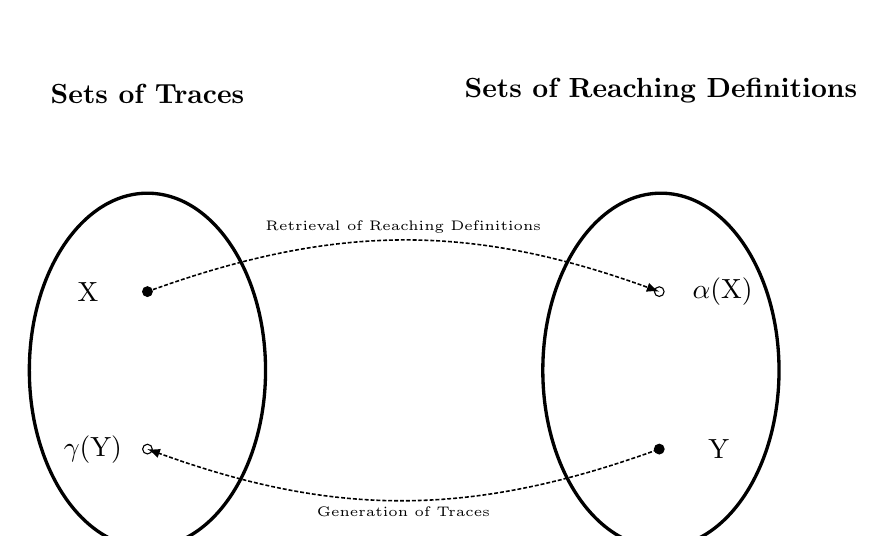
\begin{tikzpicture}
            [    
                longcircle/.style={ellipse, draw=black!100, fill=green!0, very thick, minimum width = 3cm, minimum height = 4.5cm},
                rectanglenode/.style={rectangle, draw=cyan!60, fill=cyan!20, very thick, minimum width=30mm, minimum height = 10mm},
                transparentbox/.style={rectangle,draw=blue!60, fill=blue!0, ultra thick, minimum width = 75mm, minimum height = 40mm},
            ]
            
            \node[longcircle] (main) at(0,0) {} ;
            \node[longcircle] (abstract) [right=of main] at(4,0){};

            \node [] (texttitleconcrete) [above=of main]{{\bfseries Sets of Traces}};
            \node [] (texttitleabstract) [above=of abstract]{{\bfseries Sets of Reaching Definitions}};
            

            \tkzDefPoint(0,1){traces}
            \tkzDefPoint(0,-1){reach}
            
            \tkzDrawPoints[color=black,shape=circle,fill=black,size=3.5](traces)
            \tkzDrawPoints[color=black,shape=circle,fill=black!0,size=3.5](reach)
            
            \tkzDefPoint(6.5,1){traces1}
            \tkzDefPoint(6.5,-1){reach1}
            
            \tkzDrawPoints[color=black,shape=circle,fill=black,size=3.5](reach1)
            \tkzDrawPoints[color=black,shape=circle,fill=black!0,size=3.5](traces1)
            
            \tiny
            \draw[-latex,line width=0.20mm,dashed,dash pattern=on 0.5mm off 0.25mm] (traces.140) to[bend left=(20)] node[above]{Retrieval of Reaching Definitions} (traces1.39);
            \draw[latex-,line width=0.20mm,dashed,dash pattern=on 0.5mm off 0.25mm] (reach.140) to[bend left=(-20)] node[below] {Generation of Traces} (reach1.39);
            \normalsize

            \node [] (xtext) [left=of traces] at(0.5,1) {X};
            \node [] (ytext) [left=of reach] at(0.8,-1) {$\gamma$(Y)};
            
            \node [] (xtext1) [right=of traces1] at(5.8,1) {$\alpha$(X)};
            \node [] (ytext1) [right=of reach1] at(6,-1) {Y};


        \end{tikzpicture}

        \caption{Realization of Galois Connection}
        \label{fig:realgaloisconnect}
    \end{figure}
    
    \subsection*{Induced Analysis}
    \par Finally, an induced analysis is performed on the information obtained, providing a calculated analysis of the previously undecidable properties, as shown in
    Figure \ref{fig:eptc_abstraction}. This type of analysis provides a result which is produced efficiently, and relatively precisely.

    \begin{figure}
        \centering
        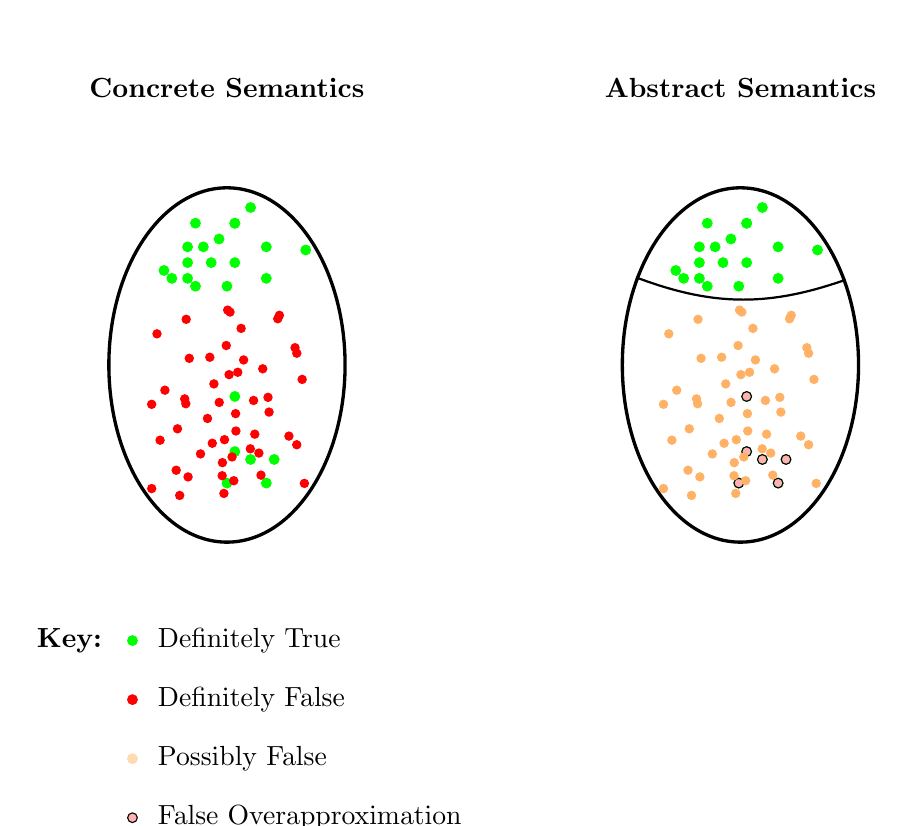
\begin{tikzpicture}
            [
                ellipsenew/.style={ellipse, draw=black!100, fill=green!0, very thick, minimum width = 3cm, minimum height = 4.5cm},
                rectanglenode/.style={rectangle, draw=cyan!60, fill=cyan!20, very thick, minimum width=30mm, minimum height = 10mm},
                transparentbox/.style={rectangle,draw=blue!60, fill=blue!0, ultra thick, minimum width = 75mm, minimum height = 40mm},
            ]

            \node[ellipsenew] (main) at(0,0) {} ;
            \node[ellipsenew] (abstract) [right=of main] at(4,0){};
            
            %% MAIN ELLIPSE
            \pgfmathsetseed{24122015}
            \begin{scope}
                \tkzDefPoint(0,1){A}
                \tkzDefPoint(0.3,2){B}
                \tkzDefPoint(-0.2,1.3){C}
                \tkzDefPoint(-0.1,1.6){D}
                \tkzDefPoint(1,1.46){E}
                \tkzDefPoint(0.1,1.8){F}
                \tkzDefPoint(0.1,1.8){G}
                \tkzDefPoint(-.4,1.8){H}
                \tkzDefPoint(-0.3,1.5){I}
                \tkzDefPoint(0.5,1.1){J}
                \tkzDefPoint(-0.5,1.1){K}
                \tkzDefPoint(0.5,1.5){L}
                \tkzDefPoint(-0.5,1.5){M}
                \tkzDefPoint(-0.5,1.3){N}
                \tkzDefPoint(-0.7,1.1){O}
                \tkzDefPoint(-0.4,1){P}
                \tkzDefPoint(-0.8,1.2){Q}
                \tkzDefPoint(0.5,-1.5){R}
                \tkzDefPoint(0.3,-1.2){S}
                \tkzDefPoint(0.1,-1.1){T}
                \tkzDefPoint(0.6,-1.2){U}
                \tkzDefPoint(0.1,-0.4){V}
                \tkzDefPoint(0.1,1.3){W}
                \tkzDefPoint(0,-1.5){X}
                \tkzDrawPoints[color=green,shape=circle,fill=green,size=3.5](A,B,C,D,E,F,G,H,I,J,K,L,M,N,O,P,Q,R,S,T,U,V,W,X)
            \end{scope}
                        
            \begin{scope}[yshift=-0.5cm]
                \pgfmathsetseed{24122015}
                %\clip(0,0) ellipse (1.5 and 4.5);
                %\clip(0,4) ellipse (1.5 and 4.5);
                \foreach \p in {1,...,50}
                { 
                    \fill[red] (1*rand,1.2*rand) circle (0.06);
                }
                
            \end{scope}

            %% ABSTRACT ELLIPSE

            \begin{scope}[xshift=6.5cm]
                \tkzDefPoint(0,1){A}
                \tkzDefPoint(0.3,2){B}
                \tkzDefPoint(-0.2,1.3){C}
                \tkzDefPoint(-0.1,1.6){D}
                \tkzDefPoint(1,1.46){E}
                \tkzDefPoint(0.1,1.8){F}
                \tkzDefPoint(0.1,1.8){G}
                \tkzDefPoint(-.4,1.8){H}
                \tkzDefPoint(-0.3,1.5){I}
                \tkzDefPoint(0.5,1.1){J}
                \tkzDefPoint(-0.5,1.1){K}
                \tkzDefPoint(0.5,1.5){L}
                \tkzDefPoint(-0.5,1.5){M}
                \tkzDefPoint(-0.5,1.3){N}
                \tkzDefPoint(-0.7,1.1){O}
                \tkzDefPoint(-0.4,1){P}
                \tkzDefPoint(-0.8,1.2){Q}
                
                \tkzDefPoint(0.5,-1.5){R}
                \tkzDefPoint(0.3,-1.2){S}
                \tkzDefPoint(0.1,-1.1){T}
                \tkzDefPoint(0.6,-1.2){U}
                \tkzDefPoint(0.1,-0.4){V}
                
                \tkzDefPoint(0.1,1.3){W}
                
                \tkzDefPoint(0,-1.5){X}

                \tkzDrawPoints[color=green,shape=circle,fill=green,size=3.5](A,B,C,D,E,F,G,H,I,J,K,L,M,N,O,P,Q,R,S,T,U,V,W,X)
                \tkzDrawPoints[color=black,shape=circle,fill=red!30,size=3.5](R,S,T,U,V,X)
            \end{scope}

            \begin{scope}[yshift=-0.5cm, xshift=6.5cm]
                \pgfmathsetseed{24122015}
                %\clip(0,0) ellipse (1.5 and 4.5);
                %\clip(0,4) ellipse (1.5 and 4.5);
                \foreach \p in {1,...,50}
                { 
                    \fill[orange!60] (1*rand,1.2*rand) circle (0.06);
                }
                
            \end{scope}

            
            \node [] (texttitleconcrete) [above=of main]{{\bfseries Concrete Semantics}};
            \node [] (texttitleabstract) [above=of abstract]{{\bfseries Abstract Semantics}};

            \draw[thick] (abstract.140) to[bend left=(-20)] (abstract.39);
            
            %% KEY
            \begin{scope}
                \node[] (key) at(-2,-3.5) {{\bfseries Key:}};
                \node[] (dtrue) [right=of key] at(-2,-3.5) {Definitely True};
                \node[] (dfalse) [right=of key] at(-2,-4.25) {Definitely False};
                \node[] (pfalse) [right=of key] at(-2,-5) {Possibly False};
                \node[] (pfalse) [right=of key] at(-2,-5.75) {False Overapproximation};

                \tkzDefPoint(-1.2,-3.5){TESTPOINT_TRUE}
                \tkzDefPoint(-1.2,-4.25){TESTPOINT_FALSE}
                \tkzDefPoint(-1.2,-5){TESTPOINT_POSFALSE}
                \tkzDefPoint(-1.2,-5.75){TESTPOINT_FALSENEGATIVE}
                \tkzDrawPoints[color=green,shape=circle,fill=green,size=3.5](TESTPOINT_TRUE)
                \tkzDrawPoints[color=red,shape=circle,fill=red,size=3.5](TESTPOINT_FALSE)
                \tkzDrawPoints[color=orange!30,shape=circle,fill=orange!30,size=3.5](TESTPOINT_POSFALSE)
                \tkzDrawPoints[color=black,shape=circle,fill=red!30,size=3.5](TESTPOINT_FALSENEGATIVE)

            \end{scope}
            
        \end{tikzpicture}
        \caption{Efficiency-Precision trade-off presented by Abstraction Interpretation}
        \label{fig:eptc_abstraction}
    \end{figure}

    \pagebreak
    \subsection{Type and Effect Systems}
    \par Type and effect systems are the amalgamation of both an Effect System and an Annotated Type System \cite[pp.17--18]{nielson2004principlesofPA}.
    In an Effect System information about what happens when an execution occurs, rendering a change the current state, is produced (ex: what exception might be raised if this execution occurs).
    In an Annotated Type system the judgements that occur describe certain properties of states, such as a variables signum. Further detail into this method of analysis will not be delved into,
    as it is out of this papers scope. A simple Type and Effect listing may be seen in Figure \ref{lst:smlcodesnippet}.

    %%TODO: Fix spacing + page
    \begin{figure}
        \centering
        {\bfseries Type \& Effect System}

        \begin{code}
            let val ref = reference (fn x=>x)   TYPE:   int -> int reference
                                                EFFECT: Creates an 
                                                        int -> int reference
            in { ref := (fn n=>n+1);                    
                !ref true    
                }
            end                                            
           
        \end{code}
        \caption{SML Code Snippet}
        \label{lst:smlcodesnippet}
    \end{figure}

\chapter{Methodology}
    \section{Abstract Design}
    \par PATH is a three-phase, 8-stage bytecode inspection tool (Sections \ref{subsec:phaseoverview} \& \ref{sec:concimp} respectively). The high-level implantation is as follows; 
    PATH iteratively inspects each bytecode instruction produced by the Python Compiler, generating facts as instructions are iterated through.
    \andre{Show i include file saving as a phase??}
        \subsection{Phase Overview}
        \label{subsec:phaseoverview}
        \begin{itemize}
            \item[1.] The preliminary phase is the setup phase. This phase tackles the initialization of all the global variables required for bytecode inspection.
            \item[2.] The second phase is the iteration phase; BIL(Bytecode Iteration Loop). This phase is where the main logic of the framework is found. The manipulation of local and global variables, pertaining to the IR and fact generation also occurs in this phase.
            \item[3.] The third and final phase generates a block summary, by pulling information from the generated facts in phase 2.   
        \end{itemize}
        
        \begin{figure}
            
            \begin{tikzpicture}
            
                [
                roundnode/.style={circle, draw=green!60, fill=green!5, very thick, minimum size=20mm},
                ellipsenew/.style={ellipse, draw=black!100, fill=green!0, very thick, minimum width = 3cm, minimum height = 4.5cm},
                rectanglenode/.style={rectangle, draw=cyan!60, fill=cyan!20, very thick, minimum width=30mm, minimum height = 10mm},
                transparentbox/.style={rectangle,draw=blue!60, fill=blue!0, ultra thick, minimum width = 75mm, minimum height = 40mm},
                ]

                %\node[rectangle]
                
            \end{tikzpicture}

            \caption{Phases of PATH}
            \label{fig:pathphases}
        \end{figure}

    \section{Concrete implementation}
    \label{sec:concimp}

    \section{}

    \section{Fact Generation}

    \section{IR Generation}

\chapter{Evaluation}

\chapter{Conclusion}


%Python becomes a more mainstream programming language, 
%\chapter{Body1}

%\section{section 1}

%\begin{definition}
%This is an example of a definition
%\end{definition}

%\begin{example}
%This is an example of an example :)
%\end{example}




%\part{Part2}
%\chapter{Body2}

%\section{section 2}
%\begin{proof}
%this is a proof
%\end{proof}


%\chapter{Conclusions}


\appendix

\chapter{Opcode Table}
\label{table:opcode_table}

\begin{tabular}{ |p{3cm}|p{3cm}|p{3cm}|  }
    \hline
    \multicolumn{3}{|c|}{Country List} \\
    \hline
    Country Name or Area Name& ISO ALPHA 2 Code &ISO ALPHA 3 \\
    \hline
    Afghanistan & AF &AFG \\
    Aland Islands & AX   & ALA \\
    Albania &AL & ALB \\
    Algeria    &DZ & DZA \\
    American Samoa & AS & ASM \\
    Andorra & AD & AND   \\
    Angola & AO & AGO \\
    \hline
\end{tabular}
%%example of the code environment
%\begin{code}
%this is some code;
%I hope you found this template useful.
%\end{code}


\bibliomatter

\bibliographystyle{abbrvurl}
 \bibliography{references}
 \cite{lutz2001programming}
 \cite{saabith2019python}
 \cite{bonta2019comprehensive}
 \cite{tensorflowTour}
 \cite{sweigart2012making}
 \cite{tiobe2022index}
 \cite{intel2013analysis}
 \cite{rice1953classes}
 \cite{moller2012static}
 \cite{van2021python}
 \cite{van1995python}
 \cite{pylint2021}
 \cite{srinath2017python}
 \cite{summerfield2007rapid}
 \cite{geurts1990abc}
 \cite{van1991interactively}
 \cite{dynamic2013typing}
 \cite{van1994python}
 \cite{zorn1990barrier}
 \cite{pedregosa2011scikit}
 \cite{forcier2008python}
 \cite{vanrossum1995python}
 \cite{bolz2009tracing}
 \cite{juneau2010definitive}
 \cite{mueller2010professional}
 \cite{ramachandra2009insight}
 \cite{aycock1998converting}
 \cite{tismer2000continuations}
 \cite{stack2011csuwm}
 \cite{intro2009algorithms}
 \cite{call2010stack}
 \cite{general2018stacks}
 \cite{pythonofficial2022docsdismodule}
 \cite{pythonofficial2022docspycode}
 \cite{landin1964mechanical}
 \cite{nielson2004principlesofPA}
\end{document}